\documentclass[fleqn]{article}
%\textwidth=6in
%\textheight=9in
%\pagestyle{empty}
\usepackage{amsmath,amssymb,amsthm,ragged2e,siunitx,graphicx,multicol,wrapfig,mathtools,parskip}
\usepackage[margin=0.7in]{geometry}
\usepackage[T1]{fontenc}
\usepackage[utf8]{inputenc}
\usepackage[dvipsnames]{xcolor}
\usepackage[export]{adjustbox}
\newtheorem{thm}{{\sc Theorem}}[section]
\newtheorem{prop}[thm]{{\sc Proposition}}
\newtheorem{cor}[thm]{{\sc Corollary}}
\newtheorem{lem}[thm]{{\sc Lemma}}
\newtheorem{df}[thm]{{\sc Definition}}

\DeclarePairedDelimiter\ceil{\lceil}{\rceil}
\DeclarePairedDelimiter\floor{\lfloor}{\rfloor}

\DeclareMathOperator{\sech}{sech}
\DeclareMathOperator{\csch}{csch}

% automatically makes new paragraphs have no indent
\setlength{\parindent}{0pt}

% new command for underscore
\newcommand{\underscore}{\underline{\hspace{1cm}}}

% this is a command for the space between asterisk or plus and the problem statement
\newcommand{\gap}{\hspace{.25cm}}

\newcommand*\colvec[1]{\begin{bmatrix*}[r]#1\end{bmatrix*}} 

% Uncomment this to write vectors bolded 
\renewcommand{\vec}[1]{\boldsymbol{#1}}

% Uncomment this to write vectors bolded AND with arrow on top
\newcommand{\avec}[1]{\overrightarrow{\boldsymbol{#1}}}
% this notation has an arrow on top of vector which is redundant if it is bolded

% Uncomment this to write vectors unbolded with long arrow on top
% \renewcommand{\vec}[1]{\overrightarrow{#1}}

% this is a command for a coefficient matrix with right-aligned entries (good for aligning negative signs)
\newcommand{\mat}[1]{\begin{bmatrix*}[r]#1\end{bmatrix*}} 

% this is a command for a coefficient matrix with center-aligned entries (good for aligning negative signs)
\newcommand{\cmat}[1]{\begin{bmatrix*}[c]#1\end{bmatrix*}} 

% this is a command for a DETERMNINANT matrix with right-aligned entries (good for aligning negative signs) (ABSOLUTE VALUE BARS)
\newcommand{\vmat}[1]{\begin{vmatrix*}[r]#1\end{vmatrix*}} 

% this is a command for black squares (useful for pivots in matrices) when already in math mode (between $ signs)
\newcommand{\bsq}{\blacksquare}






%%  environment for AUGMENTED  matrices
\newenvironment{amatrix}[1]{%
  \left[\begin{array}{@{}*{#1}{r}|r@{}}
}{%
  \end{array}\right]
}


%%% new command for Augmented BAR alone (helpful for putting augmented bar somewhere in middle of matrix)
\newcommand\aug{\fboxsep=-\fboxrule\!\!\!\fbox{\strut}\!\!\!}

% define new color (i.e. pink)
\definecolor{mypink1}{rgb}{0.858, 0.188, 0.478}

% define new color (i.e. medium green)
\definecolor{MediumGreen}{rgb}{0.1, 0.8, 0.65}

% define new color (i.e. dark purple)
\definecolor{DarkPurple}{rgb}{0.6, 0, 0.6}

% this is a command for the size of headers
\newcommand{\header}[1]{\noindent{\Large \textcolor{mypink1}{\textbf{#1}}}}

% this is a command for the size of subheaders
\newcommand{\subheader}[1]{\noindent{\large \textcolor{red}{\textbf{#1}}}}

% this is a command for answers in RED on same line with a space between problem and answer
\newcommand{\sred}[1]{\hspace{1cm} \textcolor{red}{#1}}

% this is a command for answers in RED on same line with NO space between problem and answer
\newcommand{\red}[1]{\textcolor{red}{#1}}

% this is a command for answers in PURPLE on same line with NO space between problem and answer
\newcommand{\DarkPurple}[1]{\textcolor{DarkPurple}{#1}}

% this is a command for answers in GREEN on same line with NO space between problem and answer
\newcommand{\MediumGreen}[1]{\textcolor{MediumGreen}{#1}}

% this is a command for answers in BLUE on same line with a space between problem and answer
\newcommand{\sblue}[1]{\hspace{1cm} \textcolor{blue}{#1}}

% this is a command for answers in BLUE on same line with NO space between problem and answer
\newcommand{\blue}[1]{\textcolor{blue}{#1}}


% this is a command for defining EXAMPLES
\theoremstyle{definition}
\newtheorem{exmp}{Example}[section]




\begin{document}

\centerline{\Large \bf Math Seminar Template Notes}
\centerline{\large \bf 1.1 (Visual and Geometric Proofs)}
\vspace{\baselineskip}

%\noindent \underline{\hspace{18cm}}

\header{1.1 (Visual and Geometric Proofs) } \\


\noindent\fbox{%
\parbox{\textwidth}{
\subheader{Overview} \\ 
%\vspace{0.25cm}
\textbf{\underline{Goals}} 
\begin{enumerate}
\item Construct visual/geometric arguments that explain why certain mathematical statements are true
\end{enumerate}
\vspace{.25cm}
}}

\vspace{0.2cm}


\subheader{Sum of Odd Positive Integers} 

\textbf{Ex 1:} What is $1+3+5+7+ \ldots + 95+97+99$?

\vspace{.25cm}
One way to calculate such a big sum is to look for a \underline{\hspace{3.5cm}}

\vspace{.5cm}
(a) $1+3=$

\vspace{.25cm}
(b) $1+3+5=$

\vspace{.25cm}
(c) $1+3+5+7=$

\vspace{.25cm}
(d) $1+3+5+7+9=$

\vspace{.25cm}
(e) \textbf{Discuss:} What's the pattern? 

\vspace{1cm}
(f) Can you use the pattern to calculate $1+3+5+7+ \ldots + 95+97+99$?

\vspace{2cm}

\textbf{Ex 2 (Group):} Let's try this problem in a visual way. I'm passing out some squares to each group. 
    \begin{itemize}
        \item Start by taking 1 square and place it on your table.
        \item Now take 3 more squares and arrange them ``next" to this first square to represent your answer to (a).
        \item Now take 5 more squares and arrange them ``next" to the squares you've already placed to represent the answer to (b)
        \item Keep going like this until you've gone through (d)
    \end{itemize}

\vspace{.5cm}

\textbf{Ex 3:} Finally, let's try this problem a 3rd way! I'm going to call the whole sum, $S$ and write:

\vspace{.25cm}
 %%%% template for multiple alignment points in system of equations
 $\begin{alignedat}{6}
		S &= 1 &&+ 3 &&+ 5 &&+ \ldots &&+97 &&+99 \\ \\
		S &= 99 &&+ 97  &&+ 95 &&+ \ldots  &&+ \underline{\hspace{.5cm}} &&+ \underline{\hspace{.5cm}} \\
		\end{alignedat}$


%%%
\newpage


\textbf{Ex 4 (Story Time!)} The mathematician Carl Gauss was annoying his kindergarten teacher, so his teacher gave him a problem to work on that he thought would take a while to do. The teacher asked him to compute $1+2+3+ \ldots + 99 + 100$.

\vspace{.25cm}
(a) \textbf{(Discuss):} Does the squares trick work for these numbers? 

\vspace{1cm}
(b) Use the method from Example 3 to compute this sum. 

\vspace{4cm}
\textbf{General Formula:} $\displaystyle{1+2+3+ \ldots + n = \frac{\hspace{1.5cm}}{}}$

\vspace{.5cm}

\subheader{Area of a Circle}

\textbf{Q:} How can we prove the formula for the area of a circle that $A = \underline{\hspace{1.5cm}}$?

%image aligned
%%
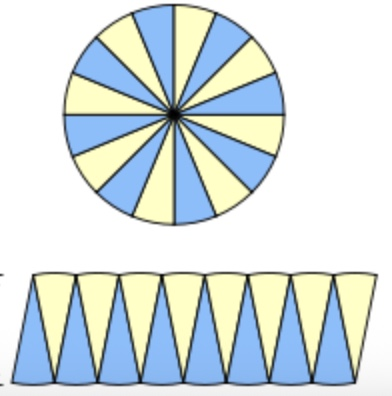
\includegraphics[scale=0.7, center]{CircleArea}

\vspace{1cm}

If we cut the circle into more and more pieces, the shape below would look more and more like a \underline{\hspace{3cm}}.

\vspace{.5cm}
Area $= \underline{\hspace{1.5cm}} = $

\vspace{.5cm}
To ``formalize" this proof we need the idea of a \underline{\hspace{2cm}} which would allow us to cut the circle into \underline{\hspace{3cm}} many pieces $\Rightarrow$ Calculus


%%%
\newpage


\subheader{Pythagorean Theorem}

\textbf{Ex 5:} In the diagram below, label the missing sides like the instructor does. 

%image aligned
%%
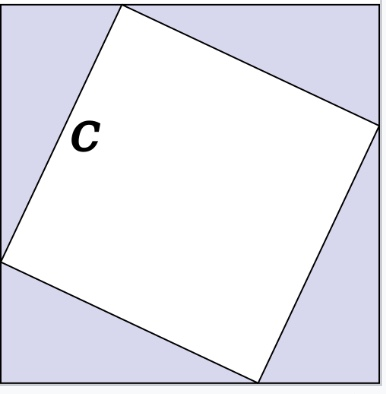
\includegraphics[scale=0.5, center]{Pythag}


\vspace{.25cm}
(a) First, let's verify that the 4-sided shape in the middle of the diagram is a square. There are 2 things we need to show to establish that it's a square. What are those 2 things?

\vspace{1.5cm}
(b) Next, let's try to show those 2 things. 

\vspace{3cm}

(c) Next, we will compute the area of the shape in 2 ways. 
    \begin{itemize}
    \item Method 1: Compute the area of the whole shape directly by finding the area of the large square
    \item Method 2: Compute the area by summing up the areas of the 4 triangles and the area of the smaller square.
    \end{itemize}

\vspace{3cm}
(d) Set the 2 expressions you got for the total area in (c) equal to each other, and simplify this expression as much as possible. 



%%%
\newpage

\subheader{Triangulation to Find Earthquake Epicenter}

\textbf{Ex 6:} Some Bay Area seismologists are trying to determine the location of a recent earthquake's epicenter. They measure the intensity of the earthquake from different sites. If location A has a higher measured intensity than location B, then location A is closer to the epicenter. If locations A and B have the same measured intensity, then they are the same distance from the epicenter. The seismologists observe that Campbell, Pleasanton, and Tiburon all had the same measured intensity for this particular earthquake.

%image aligned
%%
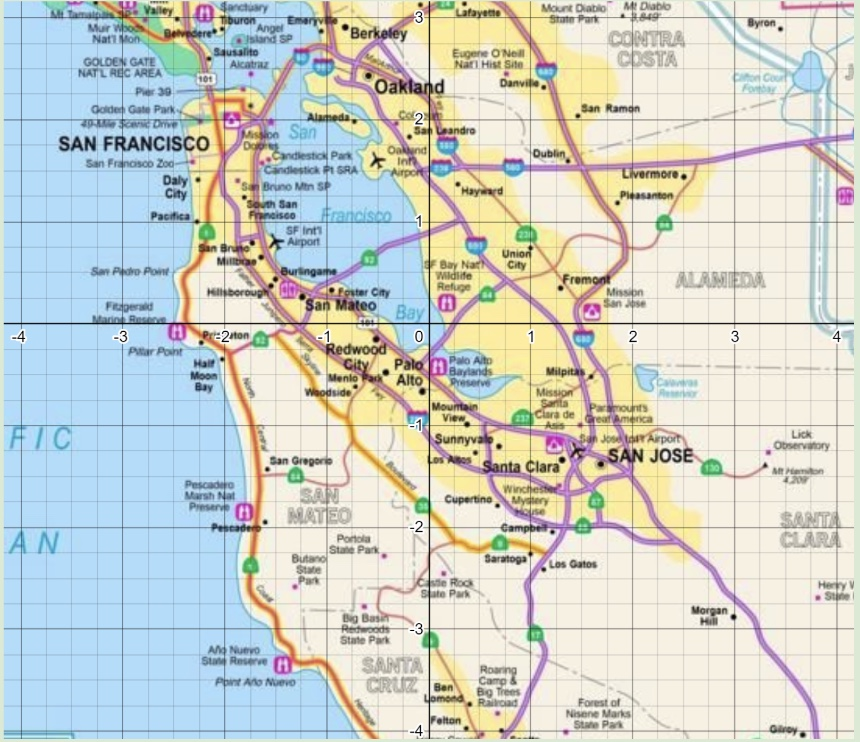
\includegraphics[scale=0.5, center]{Epicenter.jpeg}

(a) Using the xy-coordinate axes overlaid on the Bay Area map above, estimate the coordinates of Campbell, Pleasanton, and Tiburon. Round your coordinates to the nearest integer. For example, I would estimate ``Berkeley'' to be (-1, 3)

\vspace{1.5cm}
(b) Estimate where you think the epicenter is (i.e. estimate the coordinates).

%%%
\newpage
(c) Using your answers to (a), mathematically solve for the coordinates of the epicenter. (Your answer here will have fractions) What city and/or landmark is this closest to?

\vspace{15cm}
How does the epicenter relate geometrically to the points in (a)?


%%%
\newpage




\subheader{Practice Problems} 

\begin{enumerate}

\item The sum of the first n positive even integers is given by the formula:

$$2+4+6+...+2n=n(n+1)$$
% Calculate the sum for n=1,2,3, and 4.
    \begin{enumerate}
    \item Show how the proof for the sum of consecutive positive integers (the one you discussed in class using Gauss's method) could be adapted to find the sum of even integers.


\vspace{7cm}
    
    \item Visual Proof Challenge: Draw a geometric arrangement (similar to the squares used for the sum of odds, but using rectangular arrangement of dots or squares) that visually represents the proof that 2+4+6=3(3+1)=12. 
    
    \vspace{.25cm} 
    Can you keep going to construct a visual proof of this general result? 
    
    %If the last even number in a sum is 200, what is the value of the sum?
    \end{enumerate}

\vspace{3cm}
\item Fill in the blanks below for the sum of the first $n$ perfect cubes:

\vspace{.25cm}
\begin{enumerate}
\begin{multicols}{2}
\item $1^3 = \underline{\hspace{1cm}}$

\vspace{.25cm}
\item $1^3 + 2^3 = \underline{\hspace{1cm}}$

\vspace{.25cm}
\item $1^3 + 2^3 + 3^3 = \underline{\hspace{1cm}}$

\vspace{.25cm}
 $1^3 + 2^3 + 3^3 + 4^3 = \underline{\hspace{1cm}}$ \columnbreak 

 $1 = \underline{\hspace{1cm}}$

\vspace{.25cm}
 $1 + 2 = \underline{\hspace{1cm}}$

\vspace{.25cm}
 $1 + 2 + 3 = \underline{\hspace{1cm}}$

\vspace{.25cm}
 $1 + 2 + 3 + 4 = \underline{\hspace{1cm}}$
\end{multicols}

% Look back at the formula for the sum of the first n positive integers (1+2+...+n).

% \vspace{.25cm}

\item Based on the results above, hypothesize a formula for the sum of the first n cubes, $1^3+2^3+3^3+ \ldots + n^3$? 

%\vspace{.25cm}
%\textbf{Hint:} It may be helpful to look back at the formula for $1+2+3+ \ldots +n$.

 \vspace{.25cm}
(This is a famous formula that has a beautiful, albeit more complex, visual proof.)
\end{enumerate}

%%%
\newpage


\item You might remember back in algebra learning how to \textbf{complete the square} to find the vertex of a parabola (or solve a quadratic equation). For example, if we had something like $y=x^2+8x$, to complete the square we would:

\begin{itemize}
\item Divide $b=8$ by 2 to get \underline{\hspace{1cm}}
\item Square that quantity to get \underline{\hspace{1cm}}
\item Add and subtract this number. We should now have something that looks like $y= x^2 + 8x + \underline{\hspace{1cm}} - \underline{\hspace{1cm}}$
\item Finally, the first 3 terms should factor as a perfect square!
\end{itemize}

\vspace{1cm}
%image aligned
%%
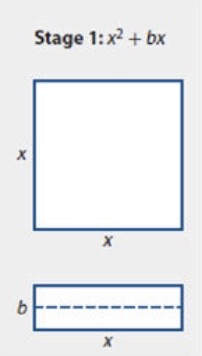
\includegraphics[scale=0.7, left]{CompleteSquare.jpeg}

In this problem, we'll construct a visual proof of why this works! 

\vspace{.25cm}
Consider the diagram which consists of a square with side length $x$ (so area is $x^2$) and a rectangle with side lengths $x$ and $b$ (so area is $bx$). 

    \begin{enumerate}
    \item Split the rectangle into 2 pieces as shown in the diagram. 
    \item Can you rearrange those 2 pieces ``next" to the square to make a shape that is ``almost" a square? 
    \item Draw in the missing shape in this new picture that would ``complete" the square. 
    \item Based on your diagram, rewrite the expression $x^2+bx$ in the form $(x + \underline{\hspace{1cm}})^2 - \underline{\hspace{1cm}}$
    \end{enumerate}


%%%
\newpage 


\item The angle bisectors of a triangle are \textbf{concurrent} (they all intersect at a single point, called the \textbf{incenter}). This point is the center of the largest circle that can be inscribed inside the triangle.

The geometric property you must use for this proof is:

\vspace{.25cm}
\fbox{{\it \textbf{Property:} Any point on the angle bisector of an angle is equidistant from the two sides of that angle.}}

\vspace{.25cm}
Follow these steps to construct the proof:

\vspace{.25cm}
\textbf{Step 1:} Draw a triangle $\Delta ABC$. 

\vspace{.25cm} 
Let $L_A$ be the angle bisector of $\angle A$ and $L_B$ be the angle bisector of $\angle B$. Let $I$ be the point where $L_A$ and $L_B$ intersect.

\vspace{1cm}

\textbf{Step 2:} Distance from Sides AB and AC: 

\vspace{.25cm}
Since $I$ is on the bisector $L_A$ of $\angle BAC$, what must be true about the distance from $I$ to side $AB$ and the distance from $I$ to side $AC$? (Use the property stated above).

\vspace{.25cm}
Let $d_1$ be the distance from $I$ to $AB$. Let $d_2$ be the distance from $I$ to $AC$.

\vspace{.25cm}
Therefore, $d_1 = d_2$. (Why?)

\vspace{1cm}
\textbf{Step 3:} Distance from Sides AB and BC: 

\vspace{.25cm}
Now do something similar to step 2 to say something about the distance from $I$ to side $AB$ and the distance from $I$ to side $BC$. 

\vspace{.25cm}
What can you conclude?

\vspace{1cm}
\textbf{Step 4:} Now combine this together and see if you can complete the proof.


\end{enumerate}




\end{document}







\begin{multicols}{5} 
Type 
\columnbreak 

Symbol 
\columnbreak

Definition 
\columnbreak

\hspace{1cm}
 \columnbreak
 
\hspace{1cm}
\end{multicols}






%%%%%%%%%%%%%%%%%%%%%%%%%%%%%%%%%%%%%%%%%%%%%%%%%%%%%%%%%




%image aligned
%%
\includegraphics[scale=0.7, right]{BlankAxes}
\vspace{-10pt}


%image centered
%%
\begin{center}
\includegraphics[scale=1.4]{SinCosTanDrawGraphs}
\end{center} 
\vspace{-20pt}



%%% incorrect/correct show something with 2 approaches
\vspace{.25cm} 
\begin{multicols}{2} 
\red{\underline{Incorrect}} \columnbreak

\MediumGreen{\underline{Correct}} 
\end{multicols}


%%% Scratch work for proof
\hspace{7cm} \MediumGreen{\underline{Scratch Work}}
\begin{multicols}{2} 
\hspace{4cm} \MediumGreen{\underline{Given/Know}} \columnbreak

\MediumGreen{\underline{Want to show}} 
\end{multicols}

\vspace{2.5cm} 



%%%% something in a box
\noindent\fbox{%
\parbox{\textwidth}{\vspace{.25cm}
\textbf{Def:} \\ (1) The \DarkPurple{intersection} of sets $A$ and $B$ is the set of all elements in \textbf{both} $A$ \textbf{and} $B$, denoted $\underline{\hspace{2cm}}$. 
\vspace{.25cm}   
}}
%%% end box


%%% big row reduction arrow
\xrightarrow{\hspace*{2cm}}  



%%% table with extra vertical spacing
\begin{tabular}{ c|c|c } 
$f'(x)$ &  $f(x)$  &  $F(x)$  \\ \hline
\rule{0pt}{3ex}           &  $x^n$  &             \\
 \rule{0pt}{5ex}          &  $\displaystyle{x^{-1}=\frac{1}{x}}$   &             \\
\rule{0pt}{5ex}           &  $e^x$  &             \\
\rule{0pt}{5ex}           &  $e^{kx}$  &             \\
\rule{0pt}{5ex}           &  $g(x) \pm h(x)$  &             \\
\rule{0pt}{5ex}           &  $cg(x)$  &             \\
\rule{0pt}{5ex}           &  $g(x)h(x)$  &             \\
\rule{0pt}{5ex}           &  $\displaystyle{\frac{g(x)}{h(x)}}$  &             \\
\end{tabular}



%%% coefficient matrix template
$A = \mat{ 1 & 0 & 1 & 2 & 2 \\ 0 & 0 & 1 & 0 & 1 \\ 2 & 0 & 1 & 4 & 3 }$


%%% augmented matrix template (the number in brackets indicates which column the augmented bar will be placed AFTER)
$\begin{amatrix}{5}
1 & -1 & 0 & -5 & 0 & -9  \\ 
0 & 0  & 1 &  4 & 0 & 4 \\ 
0 & 0  & 0 &  0 & 1 & 3  
 \end{amatrix}$
 
 
 
 %%%% template for multiple alignment points in system of equations
 $\begin{alignedat}{3}
		x_1 &+ x_2 &&- x_3 &&= -6 \\
		3x_1 &+ x_2 &&+x_3  &&= 8 \\
		4x_1 &+ 2x_2 &&      &&= 2 \\
		\end{alignedat}$
